% !TEX root =  paper.tex
\section{Results}

\begin{figure*}[t!]
	\centering
	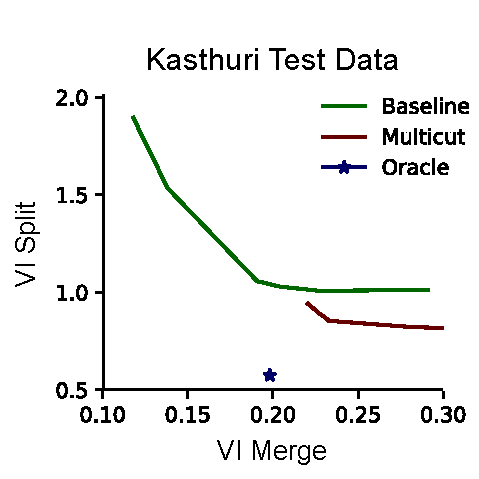
\includegraphics[width=0.32\linewidth]{./figures/benchmark/voi-Kasthuri-Luigi-Test.pdf}
	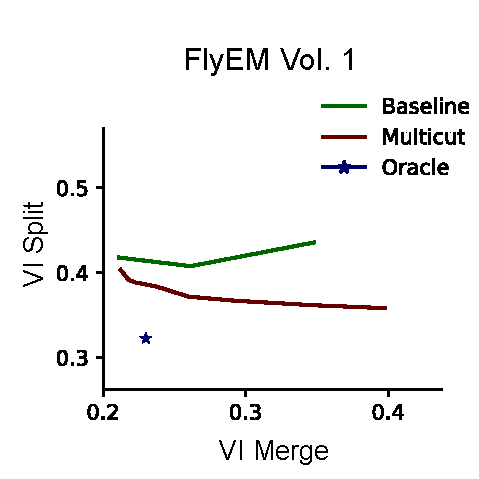
\includegraphics[width=0.32\linewidth]{./figures/benchmark/voi-FlyEM-Vol--1.pdf}
	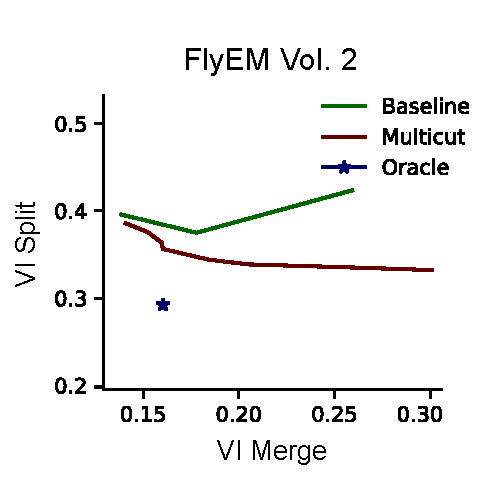
\includegraphics[width=0.32\linewidth]{./figures/benchmark/voi-FlyEM-Vol--2.pdf}
	\caption{Benchmark results on two datasets. We compare our method (red) to the baseline segmentation (green) and an oracle (blue) that optimally partitions our constructed graph as the upper-bound for our method. Lower VI scores are better. Our method improves the segmentation accuracy over the baseline in all cases.
	Note that our model is only trained on Kasthuri dataset and it generalizes well on the FlyEM dataset.}
	\label{fig:variation-of-information}
\end{figure*}

In Fig.~\ref{fig:variation-of-information}, we show the VI results of the pixel-based reconstructions of the Kasthuri and FlyEM data (Sec.~\ref{sec:dataset}) for varying thresholds of agglomeration (green). 
We use one of these segmentations (green circle) as our input dataset with an agglomeration threshold of 0.3 for all datasets. 
The results from our method are shown in red for varying the $\beta$ parameter. 
We show comparisons to an oracle (blue) that correctly partitions the graph from our method based on ground truth.

Scores closer to the origin are better for this metric, and in every instance our results are below the green curve.
We see improvements on each data with a reduction in total VI score of $10.4\%$ on the Kasthuri data and $8.9\%$ and $5.4\%$ on the FlyEM datasets.

Fig.~\ref{fig:qualitative-results} (left) shows successful merges on the Kasthuri dataset. 
Several of these examples combine multiple consecutive segments that span the volume.
In the third example on the left we correct the over-segmentation of a dendrite and attached spine-necks.
Fig.~\ref{fig:qualitative-results} (right) shows typical failure cases of our method (red circles).
In two of these examples the algorithm correctly predicts several merges before a single error renders the segment as wrong.
In the third example (blue circle) a merge error in the initial segmentation propagates to our output.
We now analyze how each major component of our method contributes to this final result.

\begin{figure}[t]
	\begin{minipage}{0.45\linewidth}
		\centering
		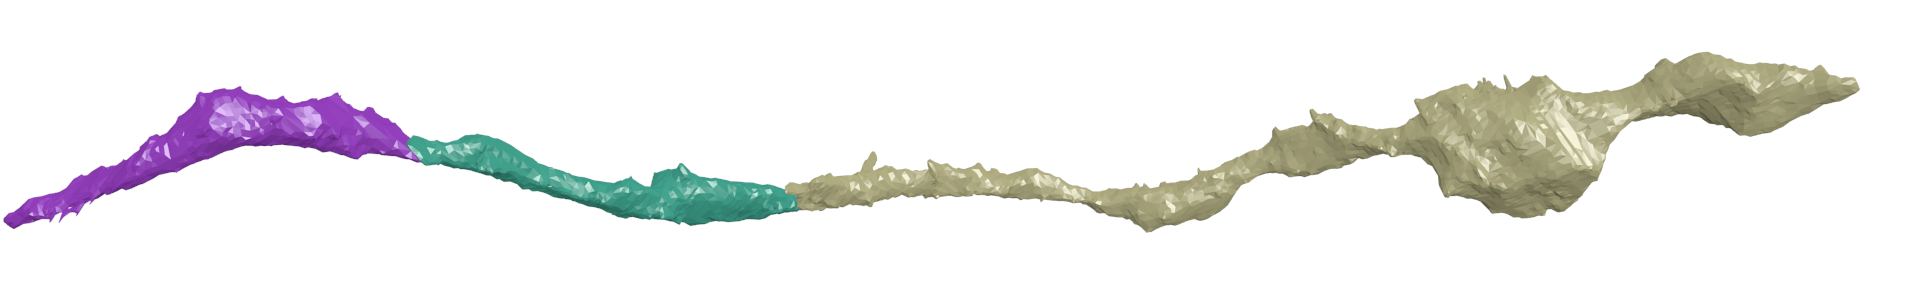
\includegraphics[width=0.85\linewidth]{./figures/VI-results/multicut-correct1.png}
		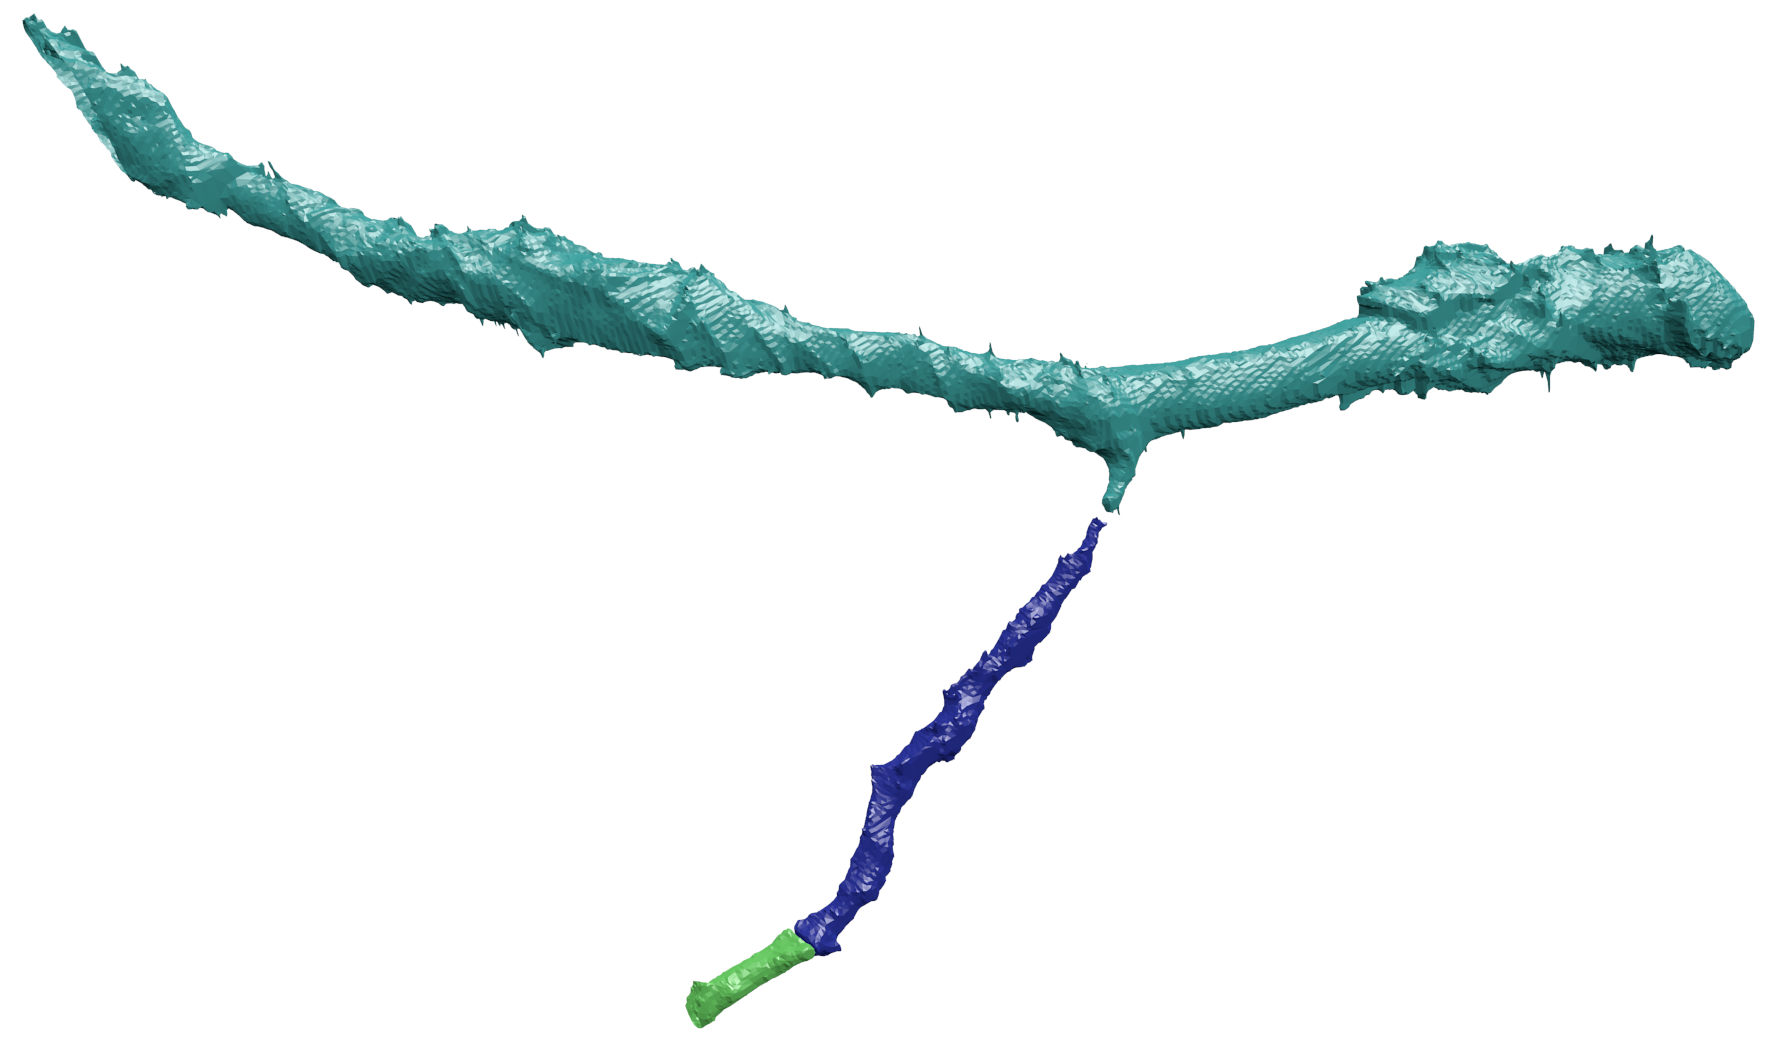
\includegraphics[width=0.85\linewidth]{./figures/VI-results/multicut-correct2.png}
		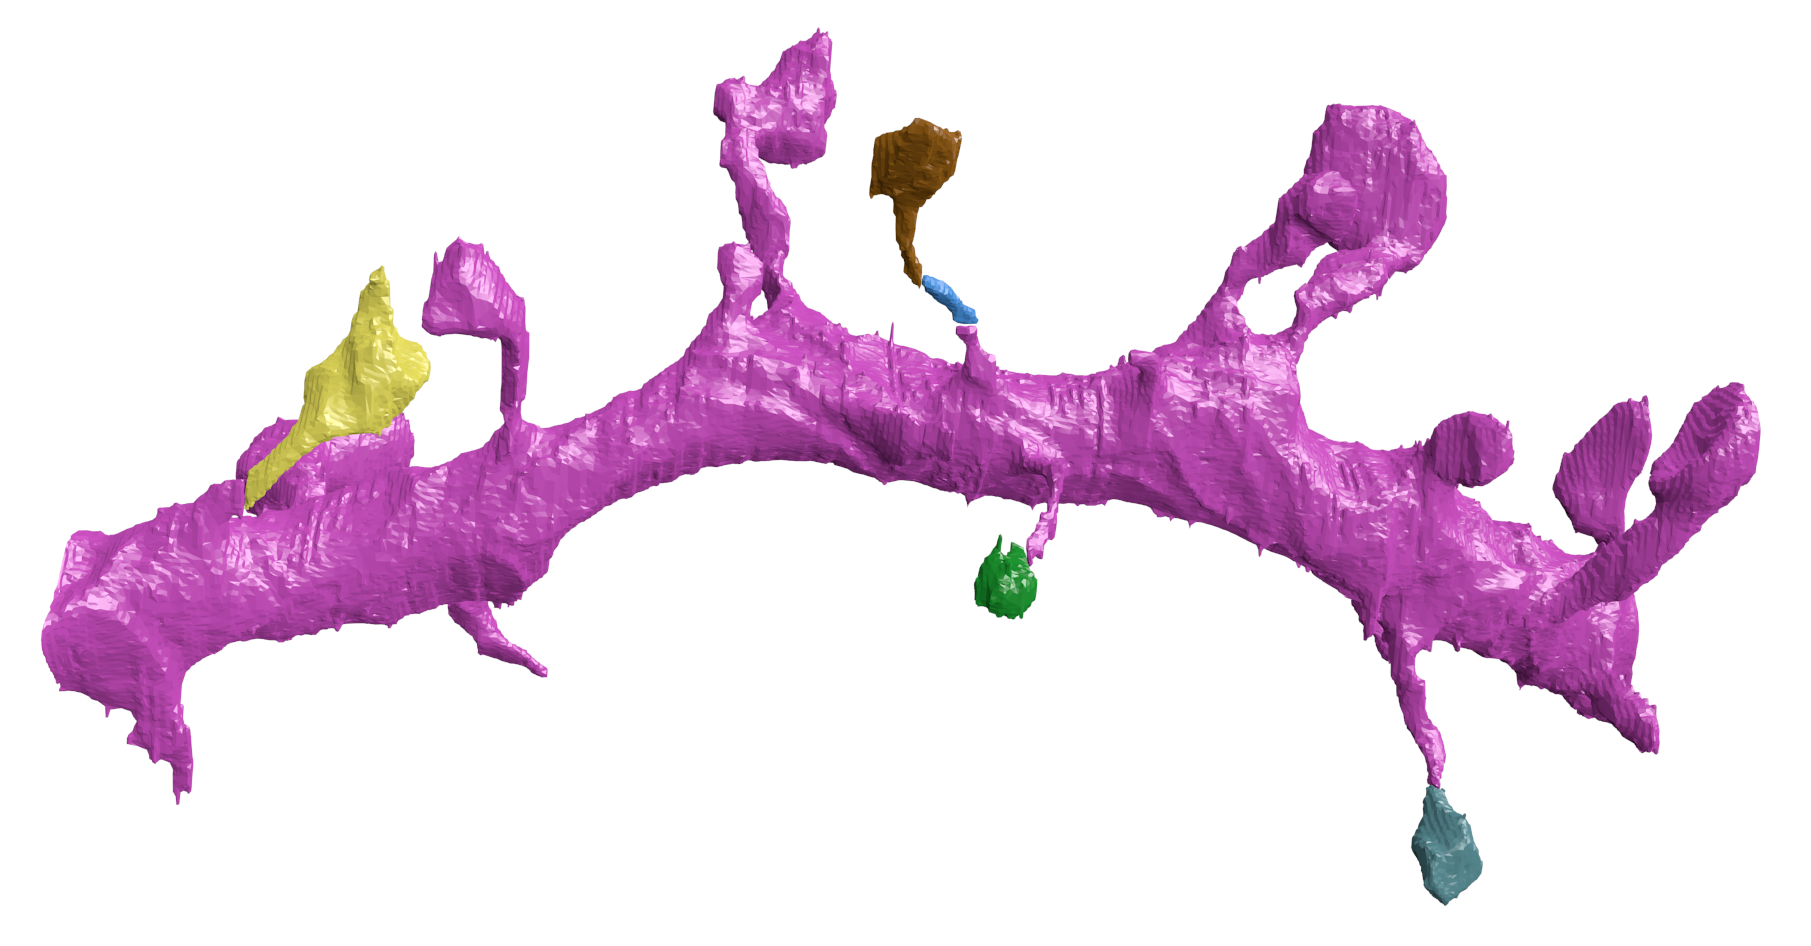
\includegraphics[width=0.85\linewidth]{./figures/VI-results/multicut-correct3.png}
		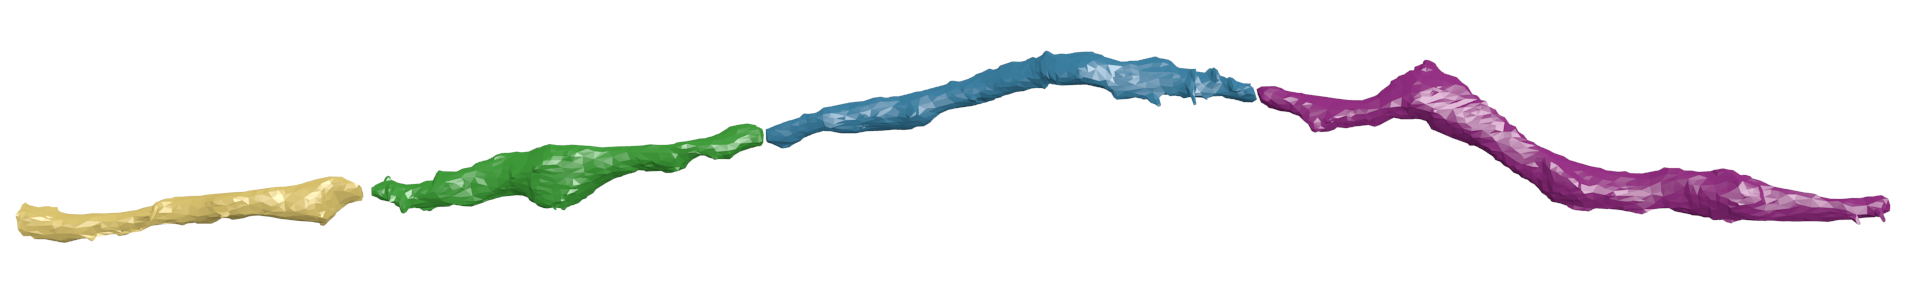
\includegraphics[width=0.85\linewidth]{./figures/VI-results/multicut-correct4.png}
		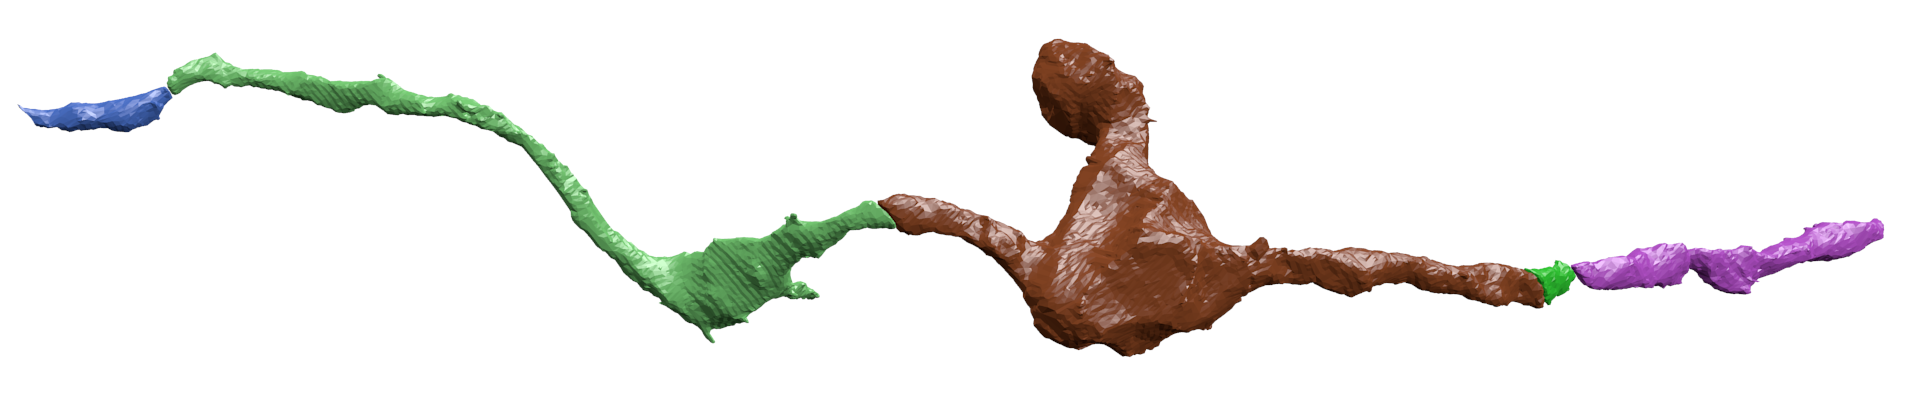
\includegraphics[width=0.85\linewidth]{./figures/VI-results/multicut-correct5.png}
	\end{minipage}
	\begin{minipage}{0.45\linewidth}
		\centering
		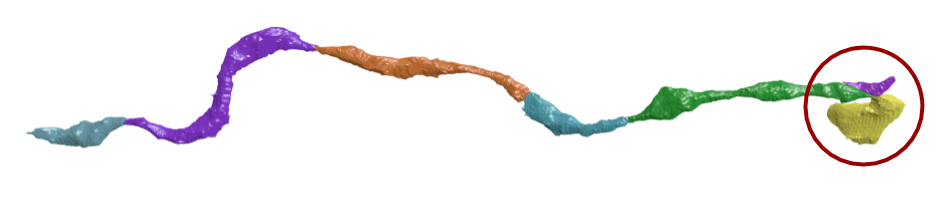
\includegraphics[width=0.85\linewidth]{./figures/VI-results/multicut-incorrect1.png}
		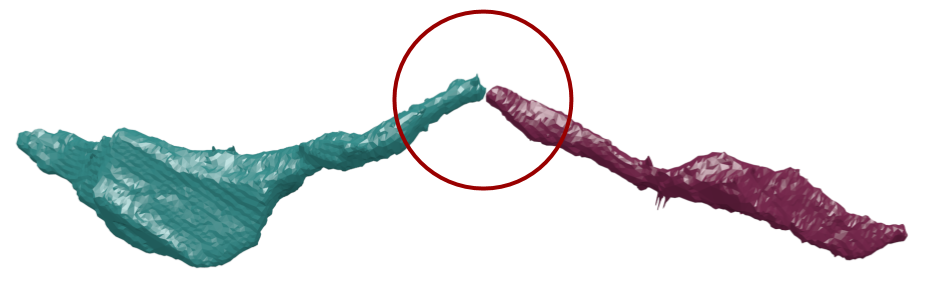
\includegraphics[width=0.85\linewidth]{./figures/VI-results/multicut-incorrect2.png}
		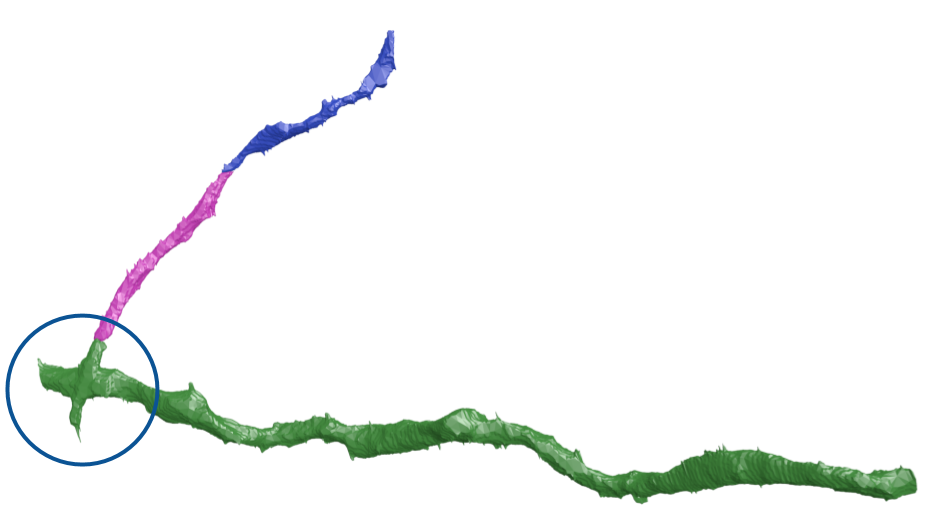
\includegraphics[width=0.85\linewidth]{./figures/VI-results/multicut-incorrect3.png}
		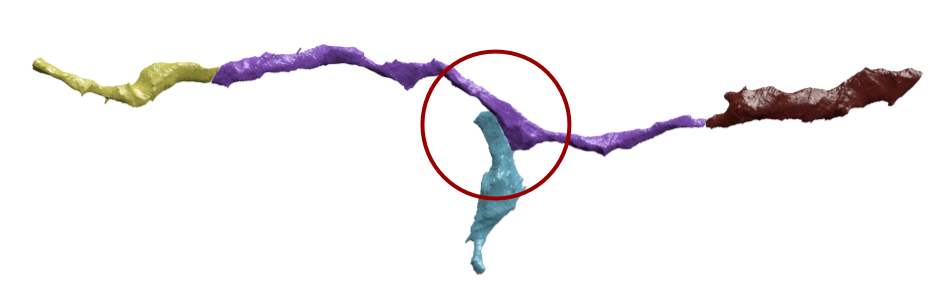
\includegraphics[width=0.85\linewidth]{./figures/VI-results/multicut-incorrect4.png}
	\end{minipage}
	\caption{(left) Segments of neurons before they were correctly merged by our method. (right) Circles indicate areas of wrong merges by our method (red) or by the initial pixel-based segmentation (blue).}
	\label{fig:qualitative-results}
\end{figure}

\subsection{Empirical Ablation Studies}

\noindent\textbf{Graph Generation.}
Table \ref{table:skeletonization} shows the results of pruning the skeleton graph using the algorithm discussed in Sec.~\ref{sec:skeletonization}. 
This edge pruning is essential for the graph partitioning algorithm, which has a non-linear computational complexity dependence on the number of edges. 
The baseline algorithm considers all adjacent regions for merging. 
Our method removes a significant portion of these candidates while maintaining a large number of the true merge locations (e.g., 764 compared to 974). 
Our pruning heuristic removes at least $3.5\times$ the number of edges on all datasets, achieving a maximum removal rate of $4.15\times$.
However, there are some adjacent over-segmented labels which are not considered. 

\begin{table}
	\caption{The results of our graph pruning approach compared to the baseline graph with all adjacent regions. We show the number of true merge locations (e.g., 974) compared to total number of edges in the graph (e.g., 25,798) for each case. The number of missed splits corresponds to the number of split errors that our method misses compared to an adjacency matrix.}
\resizebox{\linewidth}{!}{
	\begin{tabular}{c c c c c} \hline
		\textbf{Dataset} & \textbf{Segment Adjacency} & \textbf{Skeleton Pruning} & \textbf{Missed Splits} & \textbf{Gained Edges} \\ \hline
		Kasthuri & 974 / 25,798 & 764 / 6,218 & 307 & 97 \\
		FlyEM Vol. 1 & 304 / 15,949 & 212 / 4,578 & 105 & 13 \\
		FlyEM Vol. 2 &  298 / 17,614 & 197 / 4,366 & 120 & 19 \\ \hline
	\end{tabular}
}
	\centering
	\label{table:skeletonization}
\end{table}

We generate edges in our graph by using information from the skeletons. 
In particular, we do not enforce the constraint that edges in our graph correspond to adjacent segments.
Although neurons are continuous, the EM images often have noisy spots which cause an interruption in the input segmentation.
We still want to reconstruct these neurons despite the fact that the initial segmentation is non-continuous. 
The second and fourth examples in Fig.~\ref{fig:qualitative-results} show correctly reconstructed neurons where two of the segments are non-adjacent. 
\\~\\
\noindent\textbf{Failure Cases}
There are some pairs of segments which we do not consider for merging because of our reliance on the skeletons.
Fig.~\ref{fig:skeleton-results} shows two such cases with the closest endpoints circled. 
In the right example the small segment is carved from the larger segment in a location where there are no skeleton endpoints. 
There are on average 177 such examples in our datasets.
\\~\\
\noindent\textbf{Edge Weight Learning}
%\subsubsection{Inference Augmentation}
%\noindent\textbf{Inference Augmentation.}
Data augmentation at test time can improve accuracy results~\cite{lee2017superhuman,zeng2017deepem3d}.
When computing the probability to merge two segments, we randomly rotate and flip the examples three times (in the same fashion as training augmentation).
The supplemental material contains experiments showing the trade-offs between increased accuracy and runtime when using these augmentation strategies.

\begin{figure}[t!]
	\centering
	\begin{minipage}{0.45\linewidth}
		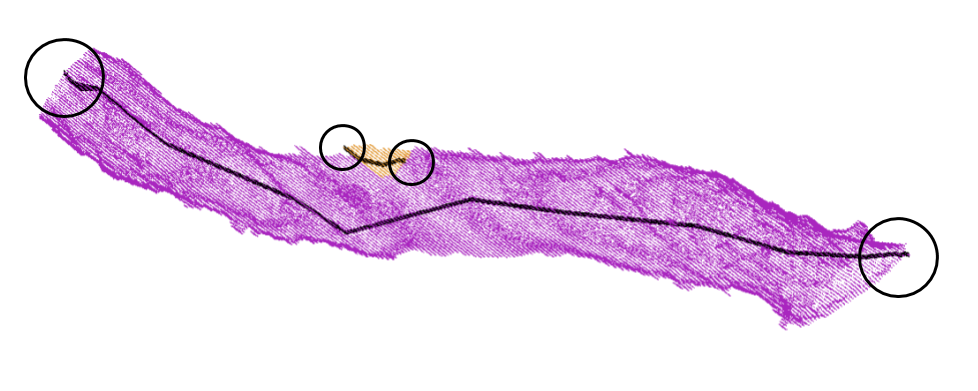
\includegraphics[width=\linewidth]{./figures/merge_candidate1.png}	
	\end{minipage}
	\hfill
	\begin{minipage}{0.45\linewidth}	
		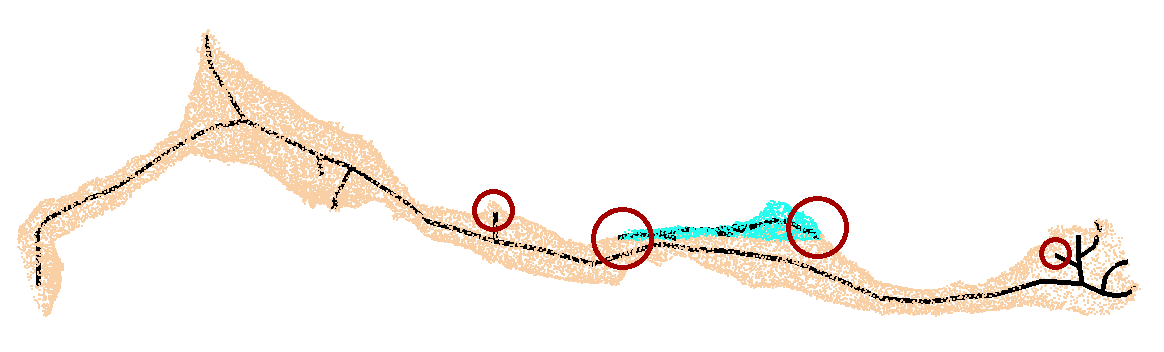
\includegraphics[width=\linewidth]{./figures/merge_candidate2.png}
	\end{minipage}
	\begin{minipage}{0.45\linewidth}
		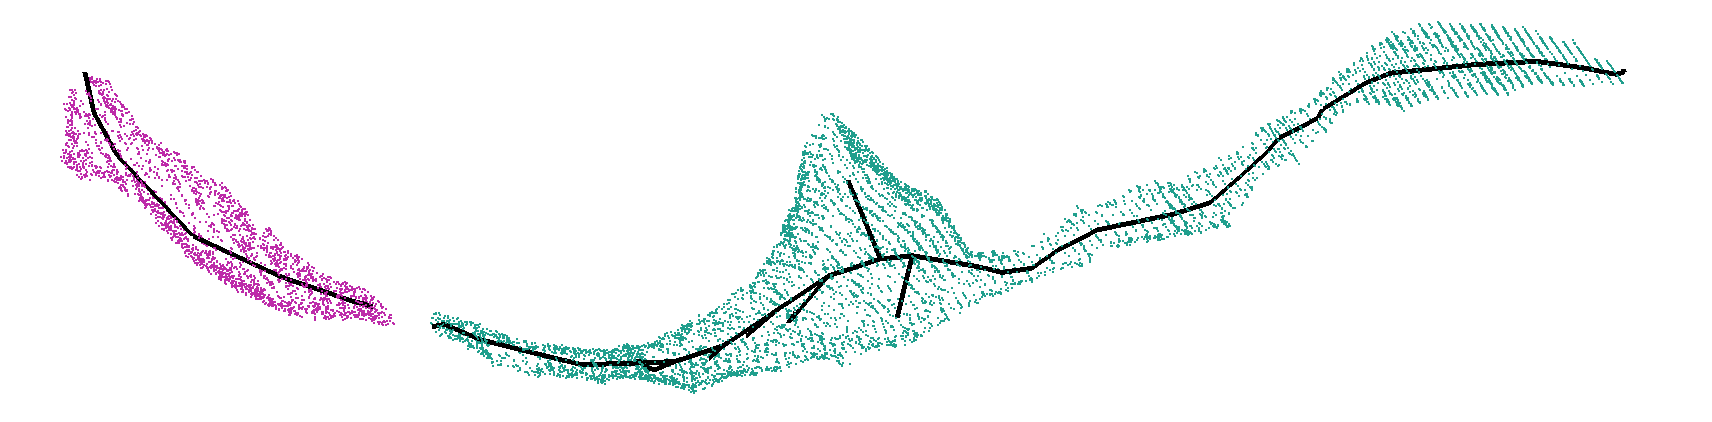
\includegraphics[width=\linewidth]{./figures/merge_candidate3.png}
	\end{minipage}
	\begin{minipage}{0.45\linewidth}
		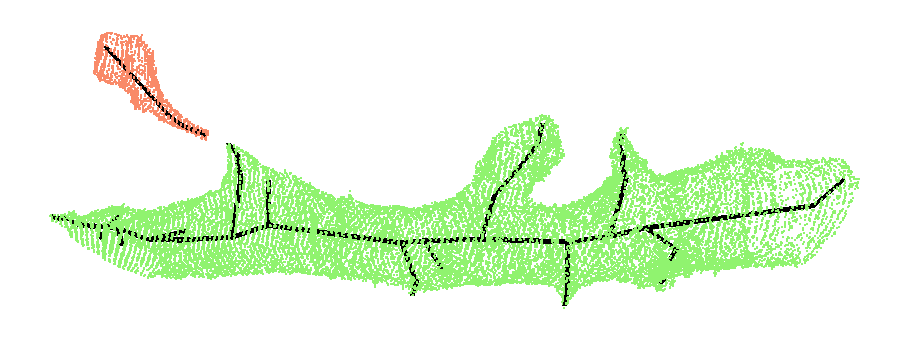
\includegraphics[width=\linewidth]{./figures/merge_candidate4.png}
	\end{minipage}
	\caption{The top two examples correspond to segment pairs that we incorrectly prune from the graph. The distance between the circled endpoints is too great. The bottom two examples show pairs of segments that belong to the same neuron but are not adjacent in the input segmentation. However, we correctly merge these pairs.}
	\label{fig:skeleton-results}
\end{figure}
Fig.~\ref{fig:receiver-operating-characteristic} shows the receiver operating characteristic (ROC) curve of our CNN classifier for all test datasets.
As shown by the ROC curve, the test results on the FlyEM data are better than the results for Kasthuri.
In part this comes from the disparity in the number of positive to negative merge candidates in the two graphs. 
The network easily classifies most of the negative examples leaving only a few difficult examples to predict.
Since there are more negative examples in relation to the positive examples in the FlyEM data, the ROC curve is greater.


\begin{figure}
	\centering
	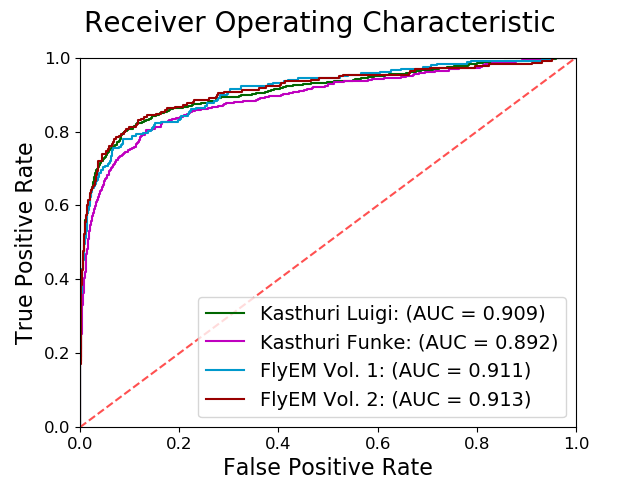
\includegraphics[width=0.45\linewidth]{./figures/receiver-operating-characteristic.png}
	\caption{The receiver operating characteristic (ROC) curves of our classifier on three connectomics datasets. The classifier works best on previously unseen data of the Kasthuri volume.}
	\label{fig:receiver-operating-characteristic}
\end{figure}

%\subsubsection{Generalization to Other Datasets}
%\noindent\textbf{Generalization to Other Datasets.}
Our neural network does not take as input the images or affinities so we can transfer network weights from one dataset to the next.
The classification results are comparable on the FlyEM datasets despite the fact that the data varies in resolution and even animal type from the training set.
\\~\\
%\subsection{Graph Optimization Results}
\noindent\textbf{Graph Partition}
The graph optimization strategy using multicut increases our accuracy over using just the CNN.
Table \ref{table:multicut} shows the changes in precision, recall, and accuracy for all four datasets compared to the CNN with both the multicut and ``lifted'' multicut formulations.
These results correspond to $\beta = 0.95$ (Sec.~\ref{sec:edge-weights}). 
The precision increases on each dataset, although the recall decreases on all but one of the datasets.
The ``lifted'' variant further accentuates this trend of increasing precision and accuracy at the expense of recall. 
Since it is more difficult to correct merge errors than split errors, it is often desirable to sacrifice recall for precision.
Over the three testing datasets, applying a graph-based partitioning strategy increased the precision by $31.9\%$, $40.9\%$, and $27.8\%$ respectively. 

\begin{table}[h]
	\caption{Precision, recall, and accuracy changes between CNN only and CNN paired with graph-optimized reconstructions for the training and three test datasets. The combined method results in better precision and accuracy. The lifted multicut extension provides very slight improvements in recall and accuracy over these three datasets.}
	\centering
\resizebox{\linewidth}{!}{
	\begin{tabular}{c c c c | c c c} \hline
		& \multicolumn{3}{c}{\textbf{Multicut}} & \multicolumn{3}{c}{\textbf{Lifted Multicut}} \\ \hline
		\textbf{Dataset} & $\Delta$ \textbf{Precision} & $\Delta$ \textbf{Recall} & $\Delta$ \textbf{Accuracy} & $\Delta$ \textbf{Precision} & $\Delta$ \textbf{Recall} & $\Delta$ \textbf{Accuracy} \\ \hline
		Kasthuri  & 31.94\% & -36.24\% & 0.71\% & -1.01\% & 0.60\% & 0.02\% \\
		FlyEM Vol. 1 & 40.87\% & -42.37\% & 1.26\% & 0.35\% & 0.85\% & 0.04\%  \\
		FlyEM Vol. 2 & 27.80\% & -44.95\% & 0.33\% & 0.54\% & 0.92\% & 0.04\% \\ \hline
	\end{tabular}
}
	\label{table:multicut}
\end{table}


\subsection{Computational Performance}
%\subsubsection{System} 
\noindent\textbf{System}
All performance experiments ran on an Intel Core i7-6800K CPU 3.40 GHz with a Titan X Pascal GPU. All code is written in Python and is freely available (link omitted for review). We use the Keras deep learning library for our neural networks with Theano backend and cuDNN 7 acceleration for CUDA 8.0.

Every step in our framework is fast enough on large connectomics datasets. 
After downsampling, skeletonization takes less than 1 second per segment on average. 
On average, each segment was skeletonized in 0.56 seconds on the training half of the Kasthuri data set. 
There are 4451 such segments resulting in a total running time of 2,492 seconds on an 800 megavoxel volume. 
From here, it took just over 31 seconds to generate the edges for our graph by considering nearby skeleton endpoints.
On our hardware, inference on the neural network had a throughput of 30 examples per second. 
Lastly, on this dataset the multicut algorithm ran for 25.28 seconds while the lifted multicut variant took 36.5 seconds.
